\documentclass[tikz,border=3pt]{standalone}
\usepackage[T1]{fontenc}
\usepackage{mathptmx}
\usepackage{pgfplots}
\pgfplotsset{compat=1.18}
\usetikzlibrary{arrows.meta}
\begin{document}
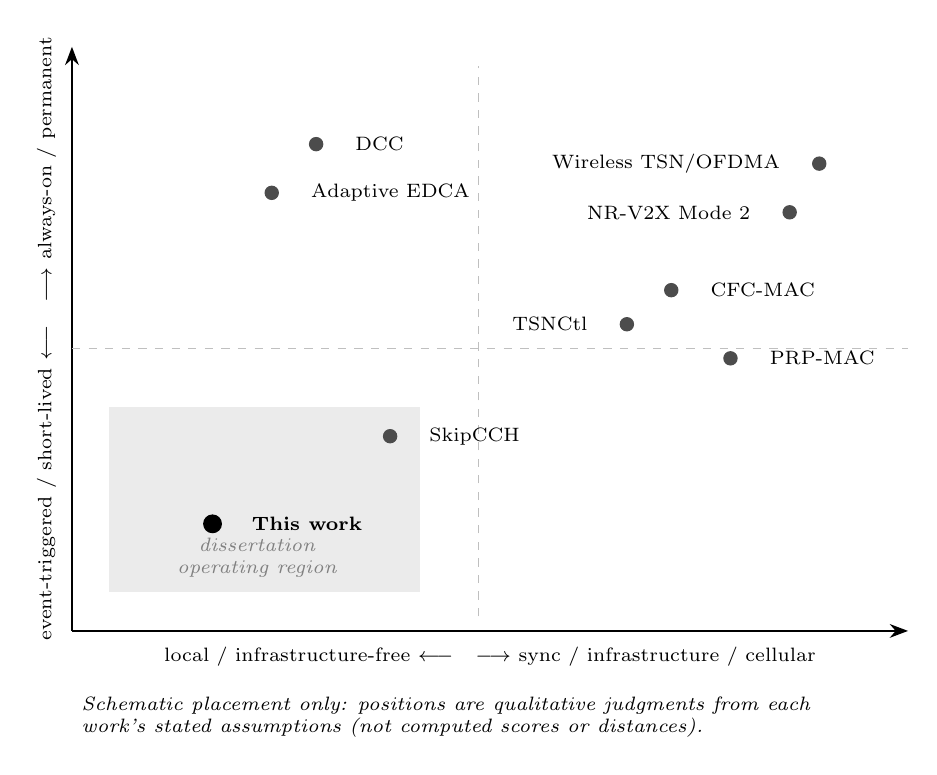
\begin{tikzpicture}
\begin{axis}[
  width=12.2cm,
  height=9.0cm,
  xmin=-0.05, xmax=1.08,
  ymin=-0.08, ymax=1.12,
  xlabel={local / infrastructure-free
          $\longleftarrow\quad\longrightarrow$
          sync / infrastructure / cellular},
  ylabel={event-triggered / short-lived
          $\longleftarrow\quad\longrightarrow$
          always-on / permanent},
  xlabel style={font=\scriptsize, align=center},
  ylabel style={font=\scriptsize, align=center},
  xtick=\empty,
  ytick=\empty,
  axis lines=left,
  axis line style={thick,-{Stealth}},
  grid=none,
  clip=false,
]
  % Light quadrant guides (not a scored grid)
  \draw[dashed, black!25] (axis cs:0.5,-0.05) -- (axis cs:0.5,1.08);
  \draw[dashed, black!25] (axis cs:-0.05,0.5) -- (axis cs:1.08,0.5);

  % Operating-point highlight (lower-left)
  \fill[black!8] (axis cs:0,0) rectangle (axis cs:0.42,0.38);
  \node[font=\scriptsize\itshape, align=center, text=black!50]
    at (axis cs:0.20,0.07) {dissertation\\operating region};

  % Qualitative placements (not computed scores)
  \addplot[only marks, mark=*, mark size=3.2pt, black] coordinates {(0.14,0.14)};
  \node[font=\scriptsize\bfseries, anchor=west] at (axis cs:0.18,0.14) {This work};

  \addplot[only marks, mark=*, mark size=2.4pt, black!70] coordinates {(0.38,0.32)};
  \node[font=\scriptsize, anchor=west] at (axis cs:0.42,0.32) {SkipCCH};

  \addplot[only marks, mark=*, mark size=2.4pt, black!70] coordinates {(0.22,0.82)};
  \node[font=\scriptsize, anchor=west] at (axis cs:0.26,0.82) {Adaptive EDCA};

  \addplot[only marks, mark=*, mark size=2.4pt, black!70] coordinates {(0.28,0.92)};
  \node[font=\scriptsize, anchor=west] at (axis cs:0.32,0.92) {DCC};

  \addplot[only marks, mark=*, mark size=2.4pt, black!70] coordinates {(0.70,0.55)};
  \node[font=\scriptsize, anchor=east] at (axis cs:0.66,0.55) {TSNCtl};

  \addplot[only marks, mark=*, mark size=2.4pt, black!70] coordinates {(0.76,0.62)};
  \node[font=\scriptsize, anchor=west] at (axis cs:0.80,0.62) {CFC-MAC};

  \addplot[only marks, mark=*, mark size=2.4pt, black!70] coordinates {(0.84,0.48)};
  \node[font=\scriptsize, anchor=west] at (axis cs:0.88,0.48) {PRP-MAC};

  \addplot[only marks, mark=*, mark size=2.4pt, black!70] coordinates {(0.92,0.78)};
  \node[font=\scriptsize, anchor=east] at (axis cs:0.88,0.78) {NR-V2X Mode 2};

  \addplot[only marks, mark=*, mark size=2.4pt, black!70] coordinates {(0.96,0.88)};
  \node[font=\scriptsize, anchor=east] at (axis cs:0.92,0.88) {Wireless TSN/OFDMA};

\end{axis}

% Explicit disclosure under the axes
\node[font=\scriptsize\itshape, align=left, anchor=north west]
  at ([yshift=-0.15cm]current axis.below south west) {%
  Schematic placement only: positions are qualitative judgments from each\\
  work's stated assumptions (not computed scores or distances).};
\end{tikzpicture}
\end{document}
